\documentclass[11pt]{article}
\usepackage{geometry}                
\geometry{letterpaper}                   

\usepackage[utf8]{inputenc}
\usepackage{graphicx}
\graphicspath{{images/}}
\usepackage{amssymb}
\usepackage{epstopdf}
\usepackage{natbib}
\usepackage{amssymb, amsmath}
\usepackage{mcode}							% package to include the code
\lstset{language=Matlab,numbers=none}				% set code language to MATLAB
\DeclareGraphicsRule{.tif}{png}{.png}{`convert #1 `dirname #1`/`basename #1 .tif`.png}
% listings print source code
\usepackage{listings}
\usepackage{pdfpages}

%% Other useful additional commands
\newcommand{\Mx}[1]{\begin{bmatrix}#1\end{bmatrix}}
\newcommand{\dd}[2]{\frac{\text{d}#1}{\text{d}#2}}
\newcommand{\DD}[2]{\frac{\text{D}#1}{\text{D}#2}}
\newcommand{\deidei}[2]{\frac{\partial#1}{\partial#2}}
\newcommand{\Lbrace}[1]{\left\{\begin{array}{ll}#1\end{array}\right.} % left brace with text
\DeclareMathOperator{\Adj}{Adj}
\renewcommand{\i}{\dot{\imath}}

% FAST COLORED TEXT
\newcommand{\blue}[1]{\textcolor{blue}{#1}}
\newcommand{\red}[1]{\textcolor{red}{#1}}
\newcommand{\green}[1]{\textcolor{green}{#1}}
\newcommand{\purple}[1]{\textcolor{purple}{#1}}
\newcommand{\olive}[1]{\textcolor{olive}{#1}}
\newcommand{\gray}[1]{\textcolor{gray}{#1}}

%\title{Mensa optimization by queue separation}
%\author{Solcà Gerson, Demicheli Samuele, Flurin Arner, Schär Alessandro}
%\date{December 2012}

\begin{document}


\thispagestyle{empty}

\begin{center}

\includegraphics[width=5cm]{ETHlogo.eps}

\bigskip


\bigskip


\bigskip


\LARGE{ 	Lecture with Computer Exercises:\\ }
\LARGE{ Modelling and Simulating Social Systems with MATLAB\\}

\bigskip

\bigskip

\small{Project Report}\\

\bigskip

\bigskip

\bigskip

\bigskip


\begin{tabular}{|c|}
\hline
\\
\textbf{\LARGE{Mensa Optimization by Queue Separation}}\\
%\textbf{\LARGE{...}}\\
\\
\hline
\end{tabular}
\bigskip

\bigskip

\bigskip

\LARGE{Solcà Gerson, Demicheli Samuele,}\\
\LARGE{ Flurin Arner, Schär Alessandro}


\bigskip

\bigskip

\bigskip

\bigskip

\bigskip

\bigskip

\bigskip

\bigskip

Zürich\\
December 2012\\

\end{center}
\newpage

%%%%%%%%%%%%%%%%%%%%%%%%%%%%%%%%%%%%%%%%%%%%%%%%%

\newpage
\section*{Agreement for free-download}
\bigskip


\bigskip


\large We hereby agree to make our source code for this project freely available for download from the web pages of the SOMS chair. Furthermore, we assure that all source code is written by ourselves and is not violating any copyright restrictions.

\begin{center}

\bigskip


\bigskip


\begin{tabular}{@{}p{3.3cm}@{}p{6cm}@{}@{}p{6cm}@{}}
\begin{minipage}{3cm}

\end{minipage}
&
\begin{minipage}{6cm}
\vspace{4mm} \large Solcà Gerson

 \vspace{\baselineskip}

\end{minipage}
&
\begin{minipage}{6cm}

\large  Demicheli Samuele

\end{minipage}

\end{tabular}

\begin{tabular}{@{}p{3.3cm}@{}p{6cm}@{}@{}p{6cm}@{}}
\begin{minipage}{3cm}

\end{minipage}
&
\begin{minipage}{6cm}
\vspace{4mm} \large Flurin Arner

 \vspace{\baselineskip}

\end{minipage}
&
\begin{minipage}{6cm}

\large Schär Alessandro

\end{minipage}

\end{tabular}

\end{center}
\newpage

%%%%%%%%%%%%%%%%%%%%%%%%%%%%%%%%%%%%%%%

% 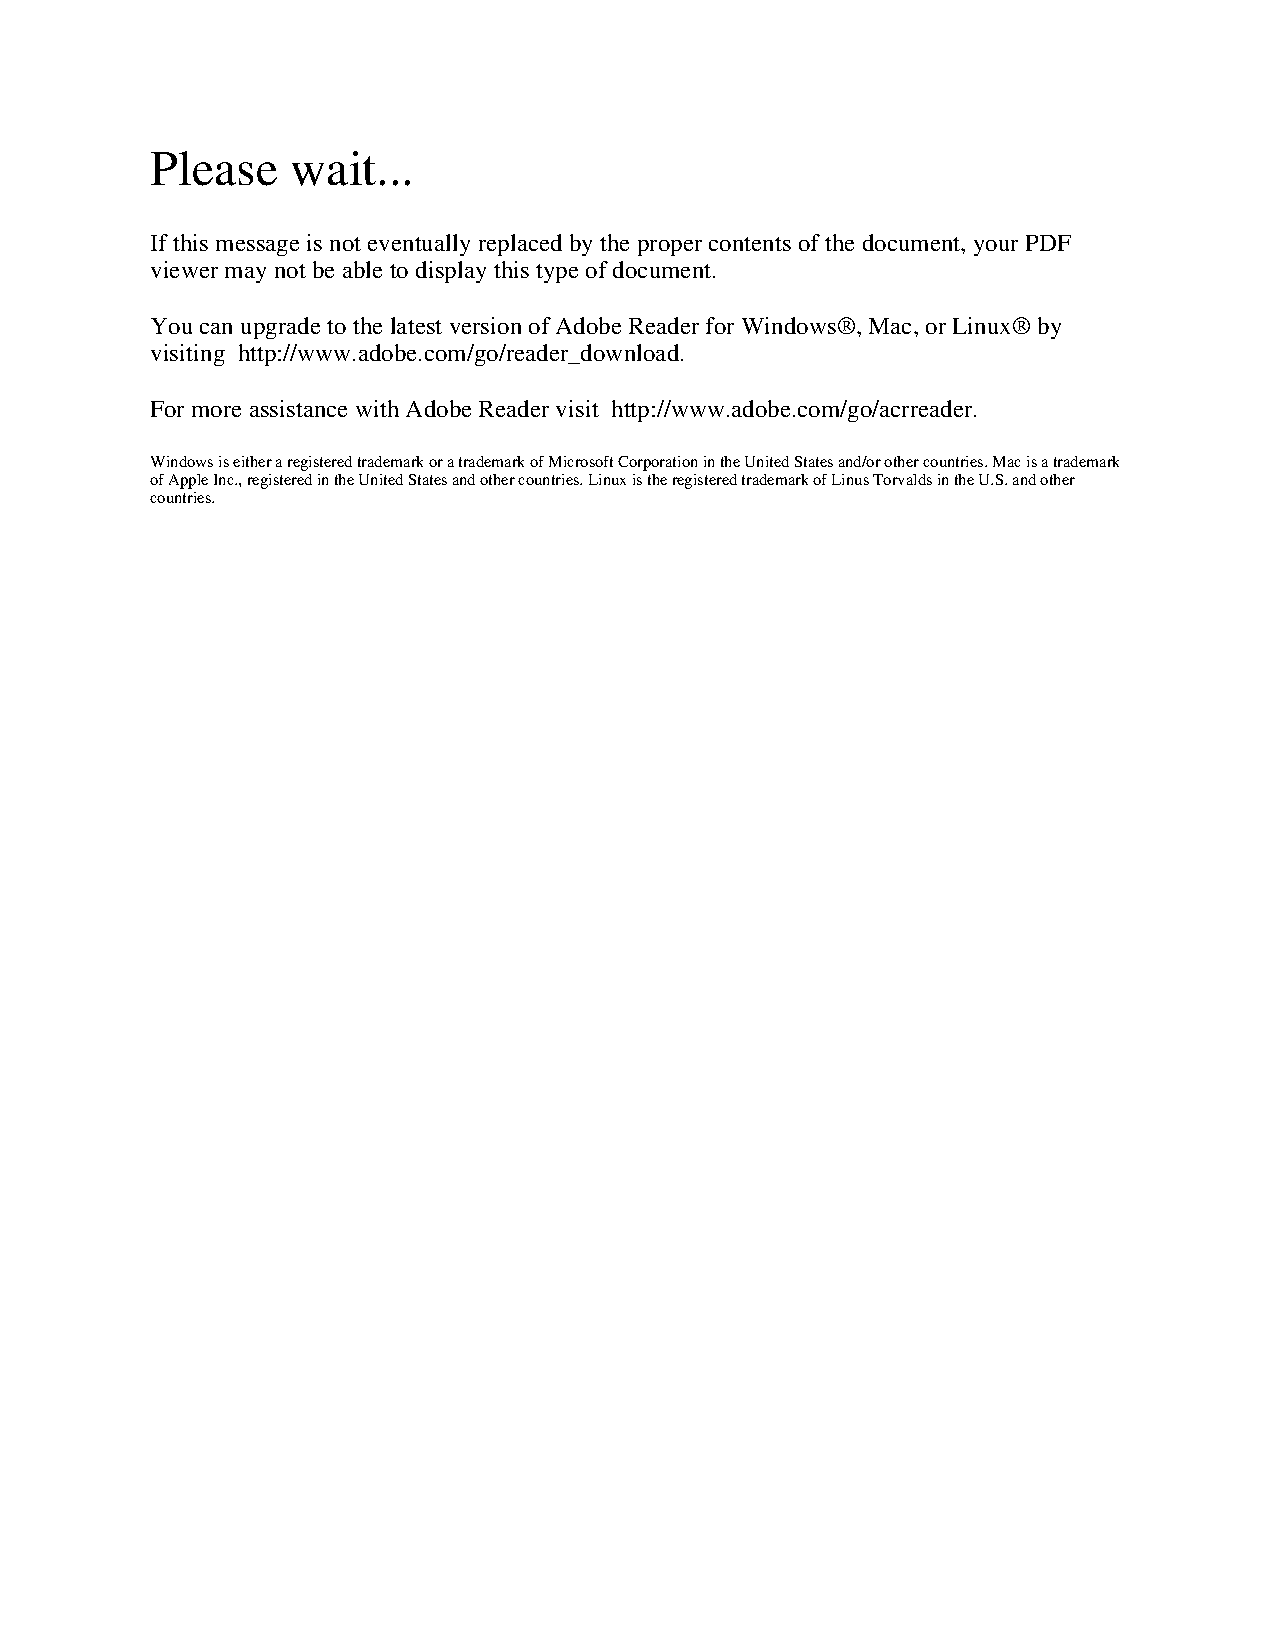
\includepdf[page=1]{confirmation_en.pdf}

\newpage

%%%%%%%%%% Table of content %%%%%%%%%%%%%%%%%

\tableofcontents

\newpage

\listoffigures

\listoftables

\newpage

%%%%%%%%%%%%%%%%%%%%%%%%%%%%%%%%%%%%%%%

\section{Abstract}

With this project we try to take a closer look at pedestrian dynamics and to study the behaviour of people in crowded places. In particular we are going to analyse the crowd that occours everyday at the ETHZ mensa and try to improve the waisted times spent waiting in queues. We generated empirical data ourselves with the help of a numerical computing sofware: MatLab$^{®}$. We built up a model based on works about the ``social force model" for pedestrian dynamics from Helbing Dirk. Other students already did a similar report about the crowd of the mensa, but our work differentiates from their in the point of view. While the other groups tried to simulate the behaviour of the crowd and to make it as real as possible trying to implement advanced real people behaviour, we used a less elaborate model to take on exam the problem of the queues itself and simulate some different scenarios by variating determined parameters in order to see if there is a solution to the daily crowd troubles.

\newpage

\section{Individual Contributions}

As a teamwork we helped each other doing the different tasks of the project, but we also devided the work in four parts, as explained in the following lines, to be more efficient. Gerson mainly cared about the report editing part: he wrote the document, the presentation and put the documents together. Samuele, Alessandro and Flurin dealed with the programming part and debugged the code. Samuele implemented the social force system, Alessandro did the initialization of the agents,  the simulition cicle and the monodimensional simulation, Flurin was responsable for the playground of our simulation; he imported the map for the visualisation, prepared the vectorfield and did a lot of debugging during the entire project.

\newpage

\section{Introduction and Motivations}

\subsection{The problem}

Everyday it's the same old story: what is an almost desert place, attended only from a couple of students or some coworkers, within a couple of minutes becomes the most crowded place of ETHZ around midday. We always have to stand and wait a long time in front of our mensa before being able to get a meal. Spend 15 or more minutes waiting in the queue is a big loose of time not only for the students but also for the other customers, this is actually a big fraction of our pause, from which one could be take advantage of in many other ways.

\subsection{The purpose}

We asked ourseves if it is possible to make this situation change, to make it better. We decided to model the structure of the canteen to see if the crowd problem was generated by its configuration. Among the huge amount of variables we could take on exam we choosed 4 listed here. 
\begin{itemize}
    \item We noticed that the lines at ETHZ canteen cross themselves, so is the path of the costumers actually playing a big role in the waiting time? And if so, is there a configuration which minimizes the walk-through-time (WTT)
    \item Is it better to have a big or a small space between the place where you get the food and the one where you pay for it?
    \item Because of the taste of the people, line waiting time can consistently alter for different meals. How does the students menus choices affect their own WTT?
    \item Is it possible that the problem lies in the employees of the canteen? Should they adopt a certain "speed pattern"? Could a perfect-constant-worker solve the queue-problem?
\end{itemize}
Will we ever be able to have a mensa without infite queues? This matter is actually the clou, the key question of this project. We aim to find a solution to it also if not practical in order to know if the crowd at the canteen is a fact that we have to accept because of the situation or it is just the most favorable scenario for those who run the canteen, because solving the problem would generate others.

\subsection{Result expectations}

Before beginning the implementation and the simulation we tought about the results that we may get from this small research about the crowd at ETHZ's canteen. We expect that the efficiency of the employees directly affects the mean WTT and that the individual effects, such as random problems that may appear on the path, may further increase the overall WTT.
 
We will come back later on tese points, after having collected the data, by the analysis to see if the result fullfilled our expectations or not, and if we were able to discover something new with this work.

We presume that sorted paths consistently etch on waiting time and different tastes affect line formation. We're going to see if this is actually the case or not

We still do not know if the problem is solvable or not, but we are going to do our best to find any useful result. 

\newpage

\section{Description of the Model}

Our model is based on Dirk Helbing's research on pedestrian dynamics, but keeps very simple. We are not taking account of the microdynamics of the mass, such as: paths formation when two or more people flows cross each other direction, social respectively antisocial behaviouror of people who form lines when waiting, or cheat trying to overtake it.

As explained in class there are mainly two ways to represent social systems, we could choose between them: the "cellular automata model" and the "social force model". We made use of the second model, since it fits better with the simulation and the purposes we have.


\subsection{The agents based model}

In opposite to the cellular automata model, that presumes a discrete space and motionless agents, the social force model takes into account a ``continuos" space where the agents interact and transfer. It is actualy impossible to reproduce a continuos space on a computer since it work with finite numbers and has no ``intelligence"; we made that by approximating a discrete space with very small parts, much smaller than the agents themselves, making the space simulation near to the continuos space, much more similar to reality. This idea is exploited in many fields such as fluiddynamics and mechanics and fits to our situation. As in fluiddynamics we're going to treat the agents as particles which are dregged from a start-region to a goal-region and, on the way, repulse each other as in real-life.

The model is really complex and can therefore take into account of many parameters. Our first idea was to be as close to reality as possible. The way we did it is described in detail in the next section.

\subsection{The social force model}

As already mentioned the agents interact with the enviroment and with each other. But how do they do it?  With how many agents does any agent iteract? This questions are pretty though to answer, but, fortunately, someone else already did the job fo us.

We based us on Dirk Helbling's research on pedestrian dynamics, so the interaction forces between the agents can be computed as follows:

\begin{equation*}
	\vec{f}_{\alpha\beta}(t) = A_\alpha^1\exp\left[\frac{r_{\alpha\beta} - d_{\alpha\beta}}{B_\alpha^1}\right]\vec{n}_{\alpha\beta}\cdot\left(\lambda_\alpha+(1-\lambda_\alpha)\frac{1+\cos(\varphi_{\alpha\beta})}{2}\right)+A_\alpha^2\exp\left[\frac{r_{\alpha\beta}-d_{\alpha\beta}}{B_\alpha^2}\right]\vec{n}_{\alpha\beta}
\end{equation*}

With:
\begin{itemize}
	\item $A_\alpha$ denotes the respective iteraction strength
	\item $B_\alpha$ denotes the range of repulsive interactions
	\item $d_{\alpha\beta}$ is the distance between the centers of masses of the pedestrians $\alpha$ and $\beta$
	\item $r_\alpha\beta$ is the sum of the radii of agents $\alpha$ and $\beta$
	\item $\vec{n}_{\alpha\beta}$ is the normalized vector pointing from $\alpha$ to $\beta$
	\item $\lambda_\alpha$ is a measure of the anisotropic nature of pedestrian interactions
\end{itemize}

Typical values [1] are
\begin{eqnarray*}
	A_\alpha^2 & = & 3 \quad\frac{\text{m}}{\text{s}^2}\\
	B_\alpha^2 & = & 0.2 \quad\text{m}\\
\end{eqnarray*}


\newpage

\section{Implementation: The Game}

\paragraph{Calculation part}
Our approach to the problem was pretty standard. We can express our solution in pseudocode as follows:
\begin{lstlisting}[frame=lines]
for i = time_interval
	for k = agents
		computeForces(k,i);
		updateVelocity(k);
		updatePosition(k);
	end
end
\end{lstlisting}
So we made at each timestep a loop over all agents, in which we computed the acting forces on the agent and updated its position according to the present forces. The details can be seen in the full version of the code.

\paragraph{Graphical part} The whole simulation was fisrt done just numerically with no visualization at all. Only in a second time, as all the simulation related computations were finished, we animated the results.

\subsection{Canteen: the playground}

\paragraph{Calculation part} The geometry of the mensa directly determines the drag force across the mensa itself. Fortunately there exists a free toolbox, which already does a major part of the job. We refer here to the Fast Marching Algorithm (FMA) which can be found at:\\
\verb"http://www.mathworks.com/matlabcentral/fileexchange/6110-toolbox-fast"\\
\verb"-marching/content/toolbox_fast_marching/html/content.html"
This toolbox is set up to take a colorcoded image with agents in their initial positions and make them move according to the social-force-agent-based-model.

Unfortunately we did not figured out how to give a changing number of agents as an input to this wonderful toolbox. More about this central problem will follow.


\paragraph{Graphical part}


To implement the map where our agents would be moving we used an helpful feature of MatLab$^{®}$. We painted the image with a simple image designer software and we imported it with the command \verb#imread()#. This command translates the image in a matrix with different values for the different colours. The different colours represented different heights/obstacles/goals, i.e. the image was a 16 color, colorcoded bitmap, in order to obtain directly the desired matrix and not a 3D array.


\subsection{People: the players}

\paragraph{Calculation part}
The players of our game were implemented as vectors, since this is the ``format" MatLab is designed for; in those vectors  were saved nine float numbers, which represented the various values that we take in account. So each agent was actually a vector of the form:
\begin{equation*}
	\vec{x} = \Mx{ID & x & y & v_x & v_y & F_{\text{des}_x} & F_{\text{des}_y} & t_\text{entering} & t_\text{exiting}}^T
\end{equation*}
Where $[\cdot]^T$ denotes the transpose operator.\\
The meaning of each term is explained in the following:
\begin{enumerate}
	\item $ID$: identification number of the agent. This value was actually used to distinguish the agents and to determine wether or not they were valid. Obviously, its value went from $1$ to the total number of simulated agents, in order to keep it as simple as possible
	\item $x$: position along the $x$-Axis (horizontal dimension)
	\item $y$: position along the $y$-Axis (vertical dimension). Since our model was 2D, we also needed two values for each parameter.
	\item $v_x$: velocity in $x$-Direction
	\item $v_y$: velocity in $y$-Direction. Even if the velocity were totally useless for the animation part, were the speed of the agents is determined by the difference of position inbetween two timesteps, we needed to save this variable for each step in order to be able to compute the next position. This can already be seen in the pseudocode above.
	\item $F_{\text{des}_x}$: ``desired" force in $x$-Direction
	\item $F_{\text{des}_y}$: ``desired" force in $y$-Direction. This two forces were those determined by the vectorfield which was estimated for the mensa from the Fast Marching Algorithm. This were the forces, which depended on the position of the agent and pushed the agents to the desired goal.
	\item $t_\text{entering}$: time at which the agent entered the mensa.
	\item $t_\text{exiting}$: time at which the agent reached the goal. This two last variables were added to the agent-vector in order to be estimated independently for each agent and at the same time to know which agent required what time. The difference between these two values gave us the ``walk-through-time" of the agent, which was the most important statistical variable of the simulation.
\end{enumerate}

There were some restrictions on certain values which had to be taken into consideration during the computation. The easiest, but most important, is that the position values $x$ \& $y$ had to be integer values, because we had a huge mensa (1000$\times$1000) and the plot only could work with points corresponding to this grid. The grid was made of steps of width 1.

The responsable code for the initialization of the agents is \verb"initAgents.m"

But how does the people arrive in time? On:\\
\verb"http://www.gastro.ethz.ch/locations/eth_zentrum/mensa/index_EN"\\
we found some interesting and useful data. Each day 2400 meals are sold for lunch, which goes from 11:15 to 13:30. Therefore we set our simulation to 9000 timesteps of 1 second each, what corresponds to a simuation-time of 2.5 hours. We then assumed that people arrive in a sort-of-gaussian way, i.e. we generated the following functions \verb"Prova_Gauss(t)" and \verb"Arriving_people(t)"

\begin{lstlisting}[frame= lines]
% 'Gaussian Distribution' function
function p = Prova_Gauss(t)
    % Define the Parameters of the Gaussian dirstribution
    mu = 1000;
    sigma = 1700;        
    A = 2/3700;
    % Values obtained by "trying"
    
    % MATLAB's DEFINITION
    % p = A*(normpdf(t,mu,sigma)+1);
    
    % People Vector as a function of time
    p=t.*A.*exp(-(t-mu).^2/(2*sigma^2));
end
\end{lstlisting}

\begin{lstlisting}[frame = lines]
% Function for the creation of the number of agents
function [people]=Arriving_people(t)
    % Local time step
    deltat = 5;

    % Number of steps
    iter = floor(length(t)/deltat);
    
    % Intializing solution vector
    compact_people = zeros(iter,1);
    people = zeros(length(t),1);
    
    % Iteration cicle (to make all the people arrive)
    for j = 1:iter
        % Temporary time vector   
        t_temp = (j-1)*deltat:j*deltat-1;
        % Filling result vector    
        compact_people(j) = floor(sum(Prova_Gauss(t_temp)));
    end
    
    % Creating time consintent people vector
    for j = 1:iter
        people(j*deltat) = compact_people(j);
    end
end
\end{lstlisting}

These two files generated the desired incoming people flow such that every 5 seconds 0,1,2,3 or 4 new agents were initialized at determined start points. The parameters \verb"mu",\verb"sigma" and \verb"A" where determined iteratively, until a plausible configuration was set. In the following image we plotted the ``continuous" output of \verb"Prova_Gauss(t)" for $t\in[0;9000]$

\begin{figure}[h]
 	\centering
		\includegraphics[width = 0.75\textwidth]{Images/GaussianDist.eps}
 	\caption{Incoming people as a continuous function of time}
  	\label{GauDis}
\end{figure}

We see that the peak is reached roughly around $t = 2500$, which corresponds to approximately 12:00, assuming the real opening times

\paragraph{Graphical part} As already mentioned, the only two values which were used in the animation were the two positions. We represented each agent as a coloured dot on the map. Obviously the coordinates of the dot were the positions $x$ \& $y$

\subsection{Forces: the rules}

\paragraph{Calculation part}
The forces that attract or reject the agents are essential for the result of the simulation. They determine the movements that every agent is going to do and therefore the path it is going to take. Of course this fact directly affects the crossing time of the guests of the mensa.
We put two kind of forces that make the agents move from the starting point to the end of the map:
\begin{enumerate}
	\item An external drag force which was determined by the geometry of the mensa, i.e. it was a vectorfield which was computed from the FMA. This force had to push the agents from the starting point to the desired goal.
	\item The repulsion forces acting on each agent due to the surrounding agents. For this force just a those agents, which were in a specific neighbourhood of the observed agent, were considered
\end{enumerate}

\paragraph{Graphical part}

Here you can see the result of the FMA on our mensa design.

\begin{figure}[h]
 	\centering
		\includegraphics[width = 0.75\textwidth]{Images/2D_IMAGES/vecField.eps}
 	\caption{Drag force vectorfield generated by the FMA}
  	\label{vecField}
\end{figure}

The white parts represent the walls, the prohibited zones whereas the arrows, obviously, represent the drag force direction in each point of the mensa. It's important to notice that we didn't use the original mensa design, but we designed our own. In our mensa there's an initial separation: the agents have to ``decide" what they want to eat (assuming each row offers a different menu) before actually entering the mensa. Therefore there's a sort of preselection.

We did not draw the forces on the map during the animation. We decided to suppress them. Althoght it would have been interesting to observe the intensity and direction of the forces in correlation with the response of the agents, the simulation would have resulted too full, maybe caotic and, moreover, it is not fundamental for the observation that we did.

\newpage
\section{Encountered Problems and Solutions}

We were mainly interested in finding a solution to the infinite queues, which form every day in the mensa. Unfortunately, the numbers we had to deal with, such as 9000 timesteps, approximately 2400 agents interacting with the enviroment and with each other, and our moderate knowledge of programming restricted our possibilities a lot.

Although, the complete simulation (2D Model) was very accurate and complex: the parameters, e.g. those mentioned just above, were took from the ``real world", the mensa was almost a continuum, etc. But this sort of model, with our computation possibilities, was way too expensive (in a computational sense) for an optimization program.

Therefore we decided to do (in addition to the compelte model) a single row simulation of the mensa, i.e. a one dimensional mensa simulation.

\subsection{The 1D Model}

\paragraph{Calculation Part}
Because it was just 1D, the agents vectors were reduced from nine to six components; all $y$-Components were eliminated. We also used a different approach for the arriving people: instead of a corrected gaussian distribution, which was used in the complete model, we decided that the people should arrive in a random way.
The arrivingPeople function was implemented as follows: 
\begin{lstlisting}[frame=lines]
function arrP = arrivingPeople(t)
    % This function tells us how many people are arriving at a certain time t
    arrP = zeros(length(t),1);
    % Let's assume that the agents arrive in a random way.
    beta = 0.5; 							% Probability tuning parameter
    for i = 1:floor(length(t)/2)
        if(rand > 0.5)
            arrP(i) = 1;
        end
    end
end
\end{lstlisting}
So if the pseudo-random value \verb"rand" was greater than \verb"beta", then a person would have arrived in that precise instant \verb"t". Setting the value of \verb"beta" to 0.5 meant that the probability of a person arriving was, according to the law of large numbers, ideally 50\%. So if one would run our simulation over a very large time interval $\Delta t$, the total number of agenst that would be simulated would be:
\begin{equation*}
	\#\text{OfAgents}_\text{TOT} = \beta\cdot\frac{1}{2}\cdot\Delta t
\end{equation*}
So in our case: $\#$OfAgents$_\text{TOT} = 0.25\cdot\Delta t$. The reason for the $\frac{1}{2}$ in the eqaution above is that we assume that people can arrive only in the first half of the time interval, so that they still have time to get out.

We also assumed that once a person has the food, he/she'll no longer be affected by the other agents, i.e. the person will continue after the bottleneck with a constant speed to its table, were he/she will finally enjoy the meal.

Instead of a 1000$\times$1000 grid we used a single 1000$\times$1 line, and the agents could only move along this axis. A very important consequence of this, was that each agent could have a maximum of two neighbours: this meant that the interaction forces that had to be comuted were less expensive, since we knew exactly which person interacted with which people.

We adapted the 2D computation to the monodimensional situation and computed the forces consequently (see code for mode detailed information)

The most important fact is that with this one dimensional model we could easily focus on the queue dynamics and analyse the walk-through time in an easier way. We also introduced an seventh agent-variable to make each agent stop for a certain time. This time is the simulation equivalent of the time needed in real-life to get the food and pay for it. We assumed that these two actions took place in the exact same spot in order to keep the simulation easy.

\paragraph{Graphical part} 
Since we only had to deal with a line it was much easier represent the mensa and the agents. In the last part of the code-file \verb"mainOneD.m" we animated the simulation by plotting a fraction of all ``active agents" at each time timestep over the whole time interval.

\begin{figure}[h]
 	\centering
		\includegraphics[width = 0.9\textwidth]{Images/RESULTS01_Stop60/oneDVideoFrame.eps}
 	\caption{A frame of the 1D Simulation animation}
  	\label{oneFrame}
\end{figure}


\section{Simulation Results and Discussion}

\subsection{Data analysis}

As mentioned above, our tuning parameter was the time needed to get the food and pay for it. We did the simulation for different values of this ``stop-time" and these were the results.
\begin{figure}[h]
 	\begin{minipage}[t]{0.48\textwidth}
		\includegraphics[width = \textwidth]{Images/RESULTS03_Stop15/PositionFracAgents.eps}
 	 \end{minipage}
  	\hfill
  	\begin{minipage}[t]{0.48\textwidth}
   		 \includegraphics[width = \textwidth]{Images/RESULTS03_Stop15/PositionAllAgents.eps}
  	\end{minipage}
  	\caption{Relative position of the agents in time for a stop time of 15s. \emph{Left}: Plot of a fraction of the agents. \emph{Right}: Plot of all the agents in time}
  	\label{img:stopTime15Agents}
\end{figure}
\begin{figure}
 	\begin{minipage}{0.48\textwidth}
		\includegraphics[width = \textwidth]{Images/RESULTS02_Stop30/PositionFracAgents.eps}
 	 \end{minipage}
  	\hfill
  	\begin{minipage}{0.48\textwidth}
   		 \includegraphics[width = \textwidth]{Images/RESULTS02_Stop30/PositionAllAgents.eps}
  	\end{minipage}
  	\caption{Relative position of the agents in time for a stop time of 30s. \emph{Left}: Plot of a fraction of the agents. \emph{Right}: Plot of all the agents in time}
  	\label{img:stopTime30Agents}
\end{figure}
\begin{figure}
 	\begin{minipage}{0.48\textwidth}
		\includegraphics[width = \textwidth]{Images/RESULTS01_Stop60/PositionFracAgents.eps}
 	 \end{minipage}
  	\hfill
  	\begin{minipage}{0.48\textwidth}
   		 \includegraphics[width = \textwidth]{Images/RESULTS01_Stop60/PositionAllAgents.eps}
  	\end{minipage}
  	\caption{Relative position of the agents in time for a stop time of 60s. \emph{Left}: Plot of a fraction of the agents. \emph{Right}: Plot of all the agents in time}
  	\label{img:stopTime60Agents}
\end{figure}

Although the number of agents treated in our simulation wasn't huge (we had a timeinterval of 1800s, so the number of agents was roughly 450), we already see some important issues regarding to the plotting of the results: all right plots show all agents involved in the corresponding simulation and the plot is very hard to read. Fortunately, we coded the plot, such that the path of each agent was plotted in a slightly different color. The consequence of this procedure is a light color gradient which makes the plots a bit clearer.
An accurate interpretation of the plots isn't still possible; therefore we decided to plot the same variables, but, instead of plotting all the involved agents, we plotted solely a fraction of them. This corresponds to the left plots.

In these left plots one sees clearly how the queue is forming in time: the gradient of the right plots translates to a ``triangle" of almost parallel lines in the left ones. A closer observation shows that the lines aren't parallel, but thei get flatened down as time passes. This is a clear sign of queue formation. It's also clear that the later an agents enter the mensa, the longer it will take to get to the goal. This fact will be analyzed and explained more in detail further below.

One may wonder why the upper halfs of all plots are almost identical. There are two main observations that have to be made regarding this:
\begin{enumerate}
	\item The upper halfs aren't identical at all! There is a specific pattern that appears with increasing stop-time (more below). As a preliminary observation, one can say that the increase of the stop-time causes a discretization/fractionalization of the outcoming people flow
	\item The lines are although all parallel because we decided that it had to be so. In fact we supposed, as already said, that the agents, once they've exit the food'n'cash region, would advance with a constant velocity to the goal.
\end{enumerate}

Note that all plots are normed in the $y$-Axis with the goal distance, i.e. we can really see how much (in percentage) a person has walked at a certain time. The $x$-Axis ist normalized, but we cut the plots at the last exiting time in order to avoid useless plot parts.

All these plots are nice and fine, but what about our variable of interest? What about the walk-through-time? We also did some graphic representations of this too and the results are pretty interesting. In the following the results of three randomly choosen results are displayed. Since the selection has been random, they shoul be representative for the model.

\begin{figure}[h]
 	\begin{minipage}{0.48\textwidth}
		\includegraphics[width = \textwidth]{Images/RESULTS03_Stop15/WalkingTimeHist.eps}
 	 \end{minipage}
  	\hfill
  	\begin{minipage}{0.48\textwidth}
   		 \includegraphics[width = \textwidth]{Images/RESULTS03_Stop15/NormalizedWalkingTimePlot.eps}
  	\end{minipage}
  	\caption{Stop-time: 15s. \emph{Left}: Histogram of the walk-through-time. \emph{Right}: Plot of the normalized walk-through-time as a function of the corresponding agent}
  	\label{img:stopTime15WTT}
\end{figure}
\begin{figure}
 	\begin{minipage}{0.48\textwidth}
		\includegraphics[width = \textwidth]{Images/RESULTS02_Stop30/WalkingTimeHist.eps}
 	 \end{minipage}
  	\hfill
  	\begin{minipage}{0.48\textwidth}
   		 \includegraphics[width = \textwidth]{Images/RESULTS02_Stop30/NormalizedWalkingTimePlot.eps}
  	\end{minipage}
  	\caption{Stop-time: 30s. \emph{Left}: Histogram of the walk-through-time. \emph{Right}: Plot of the normalized walk-through-time as a function of the corresponding agent}
	\label{img:stopTime30WTT}
\end{figure}
\begin{figure}
 	\begin{minipage}{0.48\textwidth}
		\includegraphics[width = \textwidth]{Images/RESULTS01_Stop60/WalkingTimeHist.eps}
 	 \end{minipage}
  	\hfill
  	\begin{minipage}{0.48\textwidth}
   		 \includegraphics[width = \textwidth]{Images/RESULTS01_Stop60/NormalizedWalkingTimePlot.eps}
  	\end{minipage}
  	\caption{Stop-time: 60s. \emph{Left}: Histogram of the walk-through-time. \emph{Right}: Plot of the normalized walk-through-time as a function of the corresponding agent}
  	\label{img:stopTime60WTT}
\end{figure}

Before saying anything about the plots we also show the numerical statistical values of the three data sets.

\begin{table}[h]
\begin{center}
\begin{tabular}{c|c|c|c|c}

\multicolumn{5}{c}{Statistical I}\\
\hline
\hline
Stop Time		&Mean WTT		&Standard deviation		&Max WTT	&Min WTT	\\
\hline
15s			&433.76s			&131.40s				&671s		&104s\\
\hline
30s			&524.98s			&145.71s				&748s		&120s\\
\hline
60s			&602.58s			&169.76s				&877s		&148s\\
\hline
\end{tabular}
\end{center}
\caption{Statistical data of the three showed simulations}
\end{table}
\emph{Note}: WTT $\Leftrightarrow$ Walk-Through-Time\\

The first obviuos thing to notice is, that the minimum WTT matches almost perfectly the variation of the stop-time. This is pretty logic since the first agents which enter the playground do not find any queue, so they just have to wait until the fixed time is over to procede.

We also see that as the wait time increases the standard deviation does not increase proportionally. This means that the distribution gets wider, but it doesn't get wider at the same rate that the stoptime is increased. So we can assume, that there is no such thing as a scale maintenence. This hyothesis still needs to get confirmed by larger experiments and more complex models, but, in our simple and little enviroment, this relation seems to exist over all simulations.

If we now consider the mean WTT, we see that it increases with increasing stop-time, but it follows in a certain way the behaviour of the standard deviation. This tells us that the distributions in their ensemble acts internally coherently.

On the other hand, we se how the maximum WTT doesn't follow the trend of the rest of the data. Due to the queue formation the last group of agents needs more time to get out.

Now, let's get back to the ``discretization" of the outgoing people flow. In the right plots it this phenomen becomes very clear: with increasing sotp-time the agents leave the ``food region" in more and more compact groups. For the lowest wait-time we have a sort of continuous saw profile. This profile isn't perfectly regular, but a certian periodicity is recognazible. As we increased the stop-time the profile became more and more modulated, i.e. the saw loosed half of its lines. We suppose that this is a direct effect of  the wait-time. One could probably demonstrate this effect with a more complex simulation. In the animation this phenomenon can be seen as wave packets of people.

But how does the WTT change in time? How does the right plots behave, mathematically speaking? In order to find a plausible answer to these answers, we made MatLab$^{®}$ do an appropriate fit of  a data set. This is what we got.

\begin{figure}[h]
 	\centering
		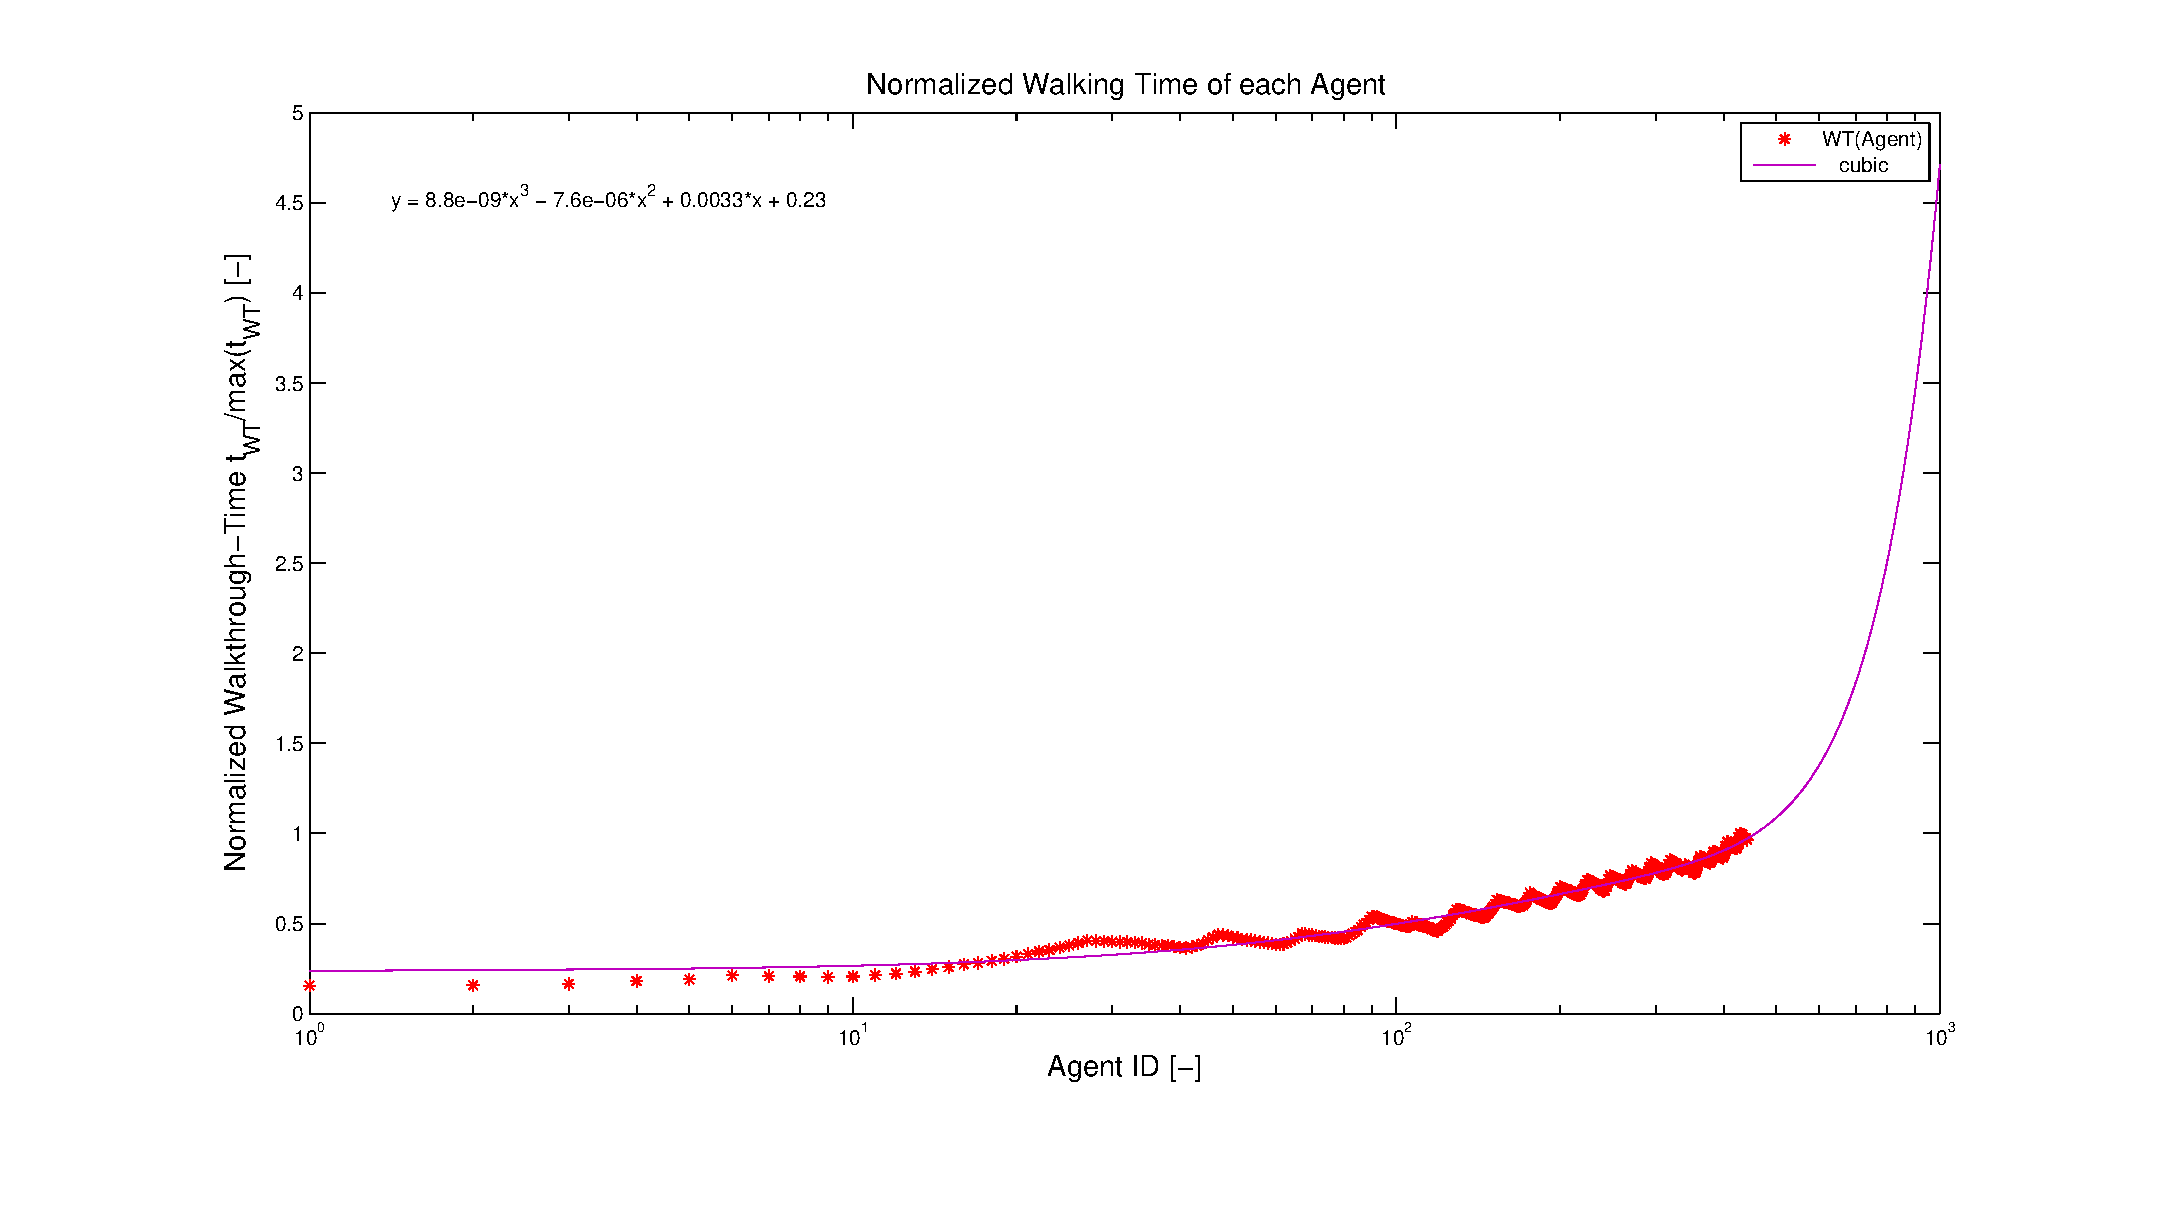
\includegraphics[width = 0.9\textwidth]{Images/walkingTimeFitting.eps}
 	\caption{WTT Cubic Fitting}
  	\label{CubicFitting}
\end{figure}
\begin{figure}
  	\centering
   		 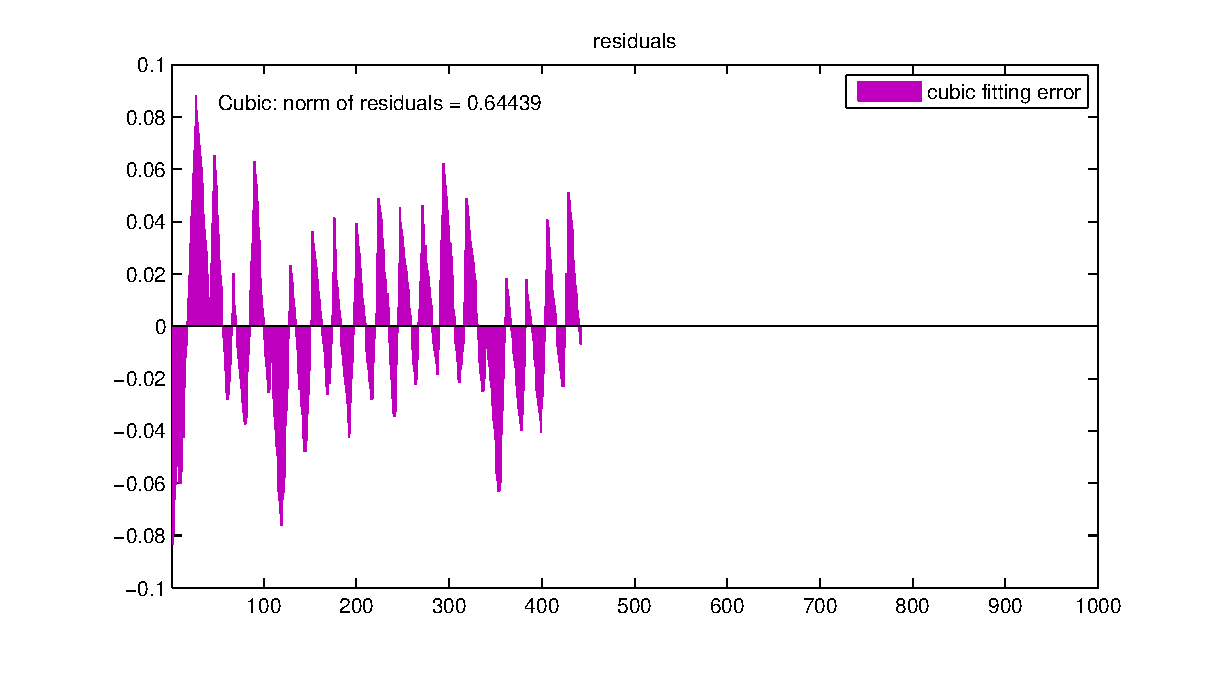
\includegraphics[width = 0.9\textwidth]{Images/cubingFittingError.eps}
  	\caption{Error of the fitting with respect to the actual data}
  	\label{FittingError}
\end{figure}

Once we had the plots we used MatLab$^{®}$'s fitting toolbox and tried different fitting types. We looked at the error to choose the best and the cubic one has turned out as the best. So if the WTTs follow the tendency they had in our simulation, the $n$-th agent's WTT could be approximately predicted by the fitting equation (cubic polynomial).

A model with constant stop time for each agent isn't 100\% realistic. So we asked ourselves the following question.
\emph{What if the wait-time of each agent is subject to a different wait-time?} We put a random time generator which was added to a minimum time of 30s. We set it such that the wait time of each agent became a value between 30s and 50s, with mean value of 40s in an ideal case. The results are showed in the following lines.

\begin{figure}[h]
 	\begin{minipage}{0.48\textwidth}
		\includegraphics[width = \textwidth]{Images/RESULTS04_RandomStop30/WalkingTimeHist.eps}
 	 \end{minipage}
  	\hfill
  	\begin{minipage}{0.48\textwidth}
   		 \includegraphics[width = \textwidth]{Images/RESULTS04_RandomStop30/NormalizedWalkingTimePlot.eps}
  	\end{minipage}
  	\caption{Stop-time: 30s + 20*rand s. \emph{Left}: Histogram of the walk-through-time. \emph{Right}: Plot of the normalized walk-through-time as a function of the corresponding agent}
  	\label{img:stopTime15WTT}
\end{figure}

We observe a little more disorder than in the previous cases. There's a sort of instability in the system which causes the normalized WTT to be more distribuited than in the previous cases.

\begin{table}
\begin{center}
\begin{tabular}{c|c|c|c|c}
\multicolumn{5}{c}{Statistics II}\\
\hline
\hline
Stop Time				&Mean WTT	&Standard deviation		&Max WTT	&Min WTT	\\
\hline
30s	$\stackrel{+0s}{+20s}$	&508.79s	&138.22s				&729s		&126s\\
\hline
\end{tabular}
\end{center}
\caption{Statistical data for random stop-time}
\end{table}

One could imagine that this visual-spread is transduced in a larger standard deviation of the WTT, but, if one looks at the data, he could observe how almost all values are smaller than those of the 30s-stop-time simulation.

\begin{table}
\begin{center}
\begin{tabular}{c|c|c|c}
\multicolumn{4}{c}{Statistics III}\\
\hline
\hline
$\Delta\bar{t}_\text{WT}$	&$\Delta \sigma_\text{WTT}$	&$\Delta t_{max}$	&$\Delta t_{min}$\\
\hline
\red{-16.19s}			&\red{-7.49s}				&\red{-55s}		&\green{+6}\\
\hline
\end{tabular}
\end{center}
\caption{Variation of the statistical data, due to randomness of the wait time}
\end{table}

As showed in the following table, the only value that follows the expectancies is the minimum WTT, which is increased by 6 seconds with respect to the 30s-stop-time simulation. The values in the already mentoined table where computed as follows:

\begin{equation*}
	\Delta\text{Measurament}_i = \text{Measurament}_{i_{RandomStopTime}} - \text{Measurament}_{i_{30sStopTime}}
\end{equation*}

Therefore a negative variation means a lower value in the simulation with increased stop time, which is against the general expectation.

But what does this mean? We can make the hypothesis that a little noise destabilizes the system, in the sense that the patterns that we recognized above are no longer regular and some exceptions are inserted. This exceptions cause a graphically more sparse distribution, but analytically we see that they cause an acceleration of most agents and this accelerations are more important than the overall larger wait-time.

\subsection{Discussion}

After the whole simulation and statistical analysis let us go back to the initial purposes to see if we reached our goals and if we can answer the questions we posed. We wanted to see what affected the WTT and try to optimize it. 

We showed that the stop-time directly affects the WTT, but it's important to notice that the relation isn't linear. So if we double the wait-time, the WTT won't double att all. So if the employees get tired during the shift and double the wait-time of the agents and the WTT of the latter doubles it's not due to the employees solely, but due to the already present queue too.

We can also say that the last mentioned results, those with wait-time of 40s$\pm$10s should be the more realistic, since the wait-time isn't a constant at all in real-life: an employee could get distracted for a short time or experience something like ``efficiency oscillations", a costumer could drop the money an have to collect it and so on. All these factors and many other affect the wait time of the single agents and therefore the queue formation and the mean WTT. \\
It's pretty straightforward that the shorter the mean stop-time is, the lower the WTT is, but the fluctuations of which we talked above really influence the overall result. This means that an irregular pattern may be better than an ideal/perfect one, if seen in terms of global results.

So, is there a way to optimize the mensa queue formation? Human errors are inveitable and random, so it might be that one day the fluctuations are such that the WTT is relatively small and, just the day after, it becomes much larger. We can say that a valid possibility os certainly to reduce the mean stop-time, but this is obviously easier to say than to do. In real-life there is such a great number of variables that have to be taken into account and that a simulation like ours can't handle that it becomes very difficult, if not impossible, to answer to the initial questions without any doubts.


\newpage
\section{Summary and Outlook}
 
We created a small crowd simulation about the canteen of ETHZ, based on the work of Helbing about pedestrian dynamics and some older reports about the same topic of the lecture `Simulating social systems with MatLab$^{®}$". We actually used a simple model compared of those from the older reports. We didn't implement some complicated mechanisms that can occur in reality, like people with social or antisocial behaviour, forming queues or trying to cut it.
In fact our goal was not to make a simulation as near as possible to reality but to try to solve, or at least to improve, the crowd problem.

As already said, we had to simplify drastically our model in order to be able to track the variation of parameters and get some significant statistical data. Therefore we reduced our huge 2D mensa to a single-row mensa and reduced the simulation time and the number of agents. This allowed us to repeat the simulation many times and to observe if there was any singularity in our simulation.

Afterwards, we analyzed the collected data of three randomly choosen simulations. We observed the ``wave-packets" formation at the exit and the expected queue formation with increasing stop-time.

We then inserted a sort of uncertainty in the stop-time, since in real-life there's no such thing as an identical wait-time over time and over all agents. Against our expectations, this fluctuations decreased the mean WTT, which was our variable of interest. So what could we conclude? Well, fluctuations of this type really appear in real life, so there is no reason to assume a model error, but we also have to consider that we choose randomly this last data set too. So, in order to assert any fundamental law of the mensa, one should first extend our 1D model to a more general an complex one and then, by analyzing a huge dataset he could, maybe, find some kind of law which rules the canteen.

Therefore, we did't actually find a close, sure answer to the questions we posed, because the time and the problems we encountered didn't allow such a huge analysis, but we have built a first milestone of what could become a much larger experiment. The time and resources aren't proportianal to the course's ones, but it should be possible to continue in this direction to find more general results.

It may be possible that a group attending this course in the future, could use our simulation files and extend them integrating some more variables and do a more profound analysis of the problem.

\newpage
\section{References}

\begin{itemize}
	\item[[1]] D. Helbing, L. Buzna, A. Johasson, T. Werner, \emph{Self-Organized Pedestrian Crowd Dynamics: Experiments, Simulations, and Design Solutions}, InfOrms, 2005.
	\item[[2]] D. Helbing, A. Johansson, \emph{Pedestrian, Crowd and Evacuation Dynamics}, pp. 6476-6495.\\
	from: http://www.ethlife.ethz.ch\%2Farchive\_articles\%2F100727\_Massenpanik\\\_Helbing\_sch\%2FPedestrian\_Crowd\_and\_Evacuation\_Dynamics\_Helbing.pdf [consulted on 14.12.2012]
	\item[[3]] P. Heer and L. B\"uhler, \emph{Pedestrian Dynamics: Airplane Evacuation Simulation}, Z\"urich, May 2011.
	\item[[4]] M. Vifian, M. Roggo, M. Aebli, \emph{Modelling Crowd Behaviour in the Plymensa Using the Social Force Model}, Z\"urich, December 2011.
\end{itemize}


\newpage

\section{Appendix A: 2D Model MatLab$^{®}$ code}

\subsection*{Arriving\_people.m}
\begin{lstlisting}[frame=lines]
% Function for the creation of the number of agents
function [people]=Arriving_people(t)
    % Local time step
    deltat = 5;

    % Number of steps
    iter = floor(length(t)/deltat);
    
    % Intializing solution vector
    compact_people = zeros(iter,1);
    people = zeros(length(t),1);
    
    % Iteration cicle (to make all the people arrive)
    for j = 1:iter
        % Temporary time vector   
        t_temp = (j-1)*deltat:j*deltat-1;
        % Filling result vector    
        compact_people(j) = floor(sum(Prova_Gauss(t_temp)));
    end
    
    % Creating time consintent people vector
    for j = 1:iter
        people(j*deltat) = compact_people(j);
    end
end
\end{lstlisting}

\subsection*{Force\_agent.m}
\begin{lstlisting}[frame= lines]
%Agent force Function
% Function that defines the force that will be applied on every agent
 %       With        
        %       agent_Matrix(:,i) = [i              (1)
        %                          Pos_xi           (2)
        %                          Pos_yi           (3)
        %                          v_xi             (4)
        %                          v_yi             (5)
        %                          ent_ti           (6)
        %                          ext_ti           (7)
        %                          des_v_xi         (8)
        %                          des_v_yi]        (9)
        
function [force_x,force_y] = Force_agent(ID,nOfAgents,AM)

%Parameters
A_1 = 1;            % interaction strength
A_2 = 1; 
B_1 = 1;            % range of repulsive interaction
B_2 = 1;          %
lamda = 0.75;       % anisotropic character of pedestrian interactions
r = 5;              % Radius of agent
epsilon = r;        % safety value to avoid divisions by 0

% Current agent
curr_A = AM(:,ID);
Pos_x = curr_A(2);
Pos_y = curr_A(3);
des_speed = [curr_A(8); curr_A(9)];         % Column Vector

% Desired force to goal
deltat = 1;     % Equals Timestep

Desired_force_x = curr_A(8)/deltat;
Desired_force_y = curr_A(9)/deltat;


% Repulsive force of agents

d_1_2 =@(x1,y1,x2,y2) sqrt((x2-x1)^2+(y2-y1)^2)+epsilon;
                                                 % Distance between centres 
                                                 % of masses
r_1_2 = 2*r;                                     % Sum of radii
n_1_2_x =@(x1,y1,x2,y2) (x2-x1+epsilon)/d_1_2(x1,y1,x2,y2);
                                                 % Normalized distance 
                                                 % vector between agents
n_1_2_y =@(x1,y1,x2,y2) (y2-y1+epsilon)/d_1_2(x1,y1,x2,y2);


e_1 =@(des_speed) des_speed/norm(des_speed);      % direction of velocity
                                                  % vector of agent 1 
phi_1_2 =@(n_1_2,e_1) acos(-1*(n_1_2'*e_1)/(norm(n_1_2)*norm(e_1)));
                                                % Angle between n_1_2 
                                                 % and e_1

Rep_force_x = zeros(nOfAgents-1,1);
Rep_force_y = zeros(nOfAgents-1,1);


for k = 1:nOfAgents
    if k~=ID
        % Helping Variable
        agent_k = AM(:,k);
        % Position of current agent is argument of function
        % Position of k'th agent
        x_k = agent_k(2);
        y_k = agent_k(3);
        posk= [x_k;y_k];
        poscurr=[Pos_x;Pos_y];
        % Calculate repulsion only for agents near our current agent
        if (norm(posk-poscurr)<6*r)
        n_1_2 = [Pos_x-x_k; Pos_y-y_k]/d_1_2(Pos_x,Pos_y,x_k,y_k);
                                            % Column Vector
        e_1A = e_1(des_speed);
        
        
        Rep_force_x(k) = A_1*exp((r_1_2-d_1_2(Pos_x,Pos_y,x_k,y_k))/...
            (B_1))*n_1_2_x(Pos_x,Pos_y,x_k,y_k)*(lamda+(1-lamda)*...
            (1+cos(phi_1_2(n_1_2,e_1A)))/2)+...
            A_2*exp((r_1_2-d_1_2(Pos_x,Pos_y,x_k,y_k))/B_2);
        Rep_force_y(k) = A_1*exp((r_1_2-d_1_2(Pos_x,Pos_y,x_k,y_k))/...
            (B_1))*n_1_2_y(Pos_x,Pos_y,x_k,y_k)*(lamda+(1-lamda)...
            *(1+cos(phi_1_2(n_1_2,e_1A)))/2)+...
            A_2*exp((r_1_2-d_1_2(Pos_x,Pos_y,x_k,y_k))/B_2);
        end
        clear x_k y_k n_1_2 e_1A;
        
    end
end
Repulsion_force_x = sum(Rep_force_x);
Repulsion_force_y = sum(Rep_force_y);

force_x = Desired_force_x + Repulsion_force_x;
force_y = Desired_force_y + Repulsion_force_y;

end
\end{lstlisting}


\subsection*{init\_agents.m}
\begin{lstlisting}[frame=lines]
% Agent initializing function
function agent_Matrix = init_agents(nOfPeople)
    % Initialize Matrix as a empty array of structs
    agent_Matrix = zeros(9,nOfPeople);
    
    % ELEMENTS OF agent_Matrix ARE VECTORS CONTAINING THE INFORMATION OF
    % THE AGENT i
    %
    %   agent_Matrix(:,i) = [ID(i) 
    %                      Pos_x(i)
    %                      Pos_y(i)
    %                      v_x(i)
    %                      v_y(i)
    %                      ent_t(i)
    %                      ext_t(i)
    %                      des_v_x(i)
    %                      des_v_y(i)]
 
    % Fill the agent_Matrix with ordered agents, i.e. set the ID's
    for i = 1:nOfPeople;
        agent_Matrix(1,i) = i; 
    end

end
\end{lstlisting}

\subsection*{main.m}

\begin{lstlisting}[frame=lines]
%% Mensa Simulation

% Group Name:     Hungry People
% Group Members:  Flurin Arner
%                 Samuele Demicheli
%                 Alessandro Schaer
%                 Gerson Solca'
%                 
% This file executes the simulation calling all the other implemented 
% functions

clear all; close all; clc;

%% Parameters

% Define the time interval in which we want to simulate
t = 0:410;             % -> We simulate 2.5 hours. Simulation step: 1s
t_F = t(length(t));         % Final Time of Simulation
% Desired velocity matrix
 global desVel_x;
 global desVel_y;
 
% Potential boundary
global V_b;

fprintf('Getting Vectors and Image...\n')
[desVel_x, desVel_y,rowW,colW,rowE,colE] = rdImggetVct();

% Define treshold y value for goal (read plausible value from the map)
y_goal = 98;

fprintf('Computing total amount of agents...\n\n');

% Vector contianing the arriving people as a gaussian distr. over time
incoming_people = Arriving_people(t);

% Total people coming during the whole time interval:
tot_people = sum(incoming_people);
fprintf('Total amount of agents is: %.f\n',tot_people);

fprintf('Over a time interval of %.f seconds.\n\n',t_F);

% Define variable which we're interested in
global walking_time;
walking_time = zeros(tot_people,1);

%% Agent Initialization
fprintf('Initializing agents...\n\n');
% Initialize the agent Matrix AM:
AM = init_agents(tot_people);
% ELEMENTS OF agent_Matrix ARE VECTORS CONTAINING THE INFORMATION OF
% THE AGENT i
%
%   agent_Matrix(:,i) = [i          
%                      Pos_xi
%                      Pos_yi
%                      v_xi
%                      v_yi
%                      ent_ti
%                      ext_ti
%                      des_v_xi
%                      des_v_yi]
fprintf('Initialization done.\n\n')

%% Actual Simulation
fprintf('################# \nStarting Simulation. \n');
fprintf('################# \n\n');
fprintf('Computing time iterations. Please be patient: ');
fprintf('the procedure \nmay take a few minutes...\n\n');

% Initialize log matrix: each time step status gets saved here
log_Matrix = cell(t_F+1,1);

% Log the arrived people
arrived_people = 0;

for i = 0:t_F-1;
   % Update log:
    arrived_people = sum(incoming_people(1:i+1));
    arrived_people_new = arrived_people + incoming_people(i+2);
   
   
   % Make appear agents as suggested by incoming_people
   % RELEVANT AGENTS HAVE A x-POSITION UNEQUAL 0!
   if(arrived_people_new ~= arrived_people)
       % Set initial positions of new agents to valid position
       for k = arrived_people+1:arrived_people_new;
            updatingAgent = AM(:,k);
            % Initialize x-Position as 499,500,501 or 502 (in the middle of
            % the mensa map along the y=10-Axis) 
            updatingAgent(2) = 48+k-arrived_people;
            
            % y-Position to 10
            updatingAgent(3) = 10;
            
            % Set des velocity
            updatingAgent(8) = desVel_x(updatingAgent(2),updatingAgent(3));
            updatingAgent(9) = desVel_y(updatingAgent(2),updatingAgent(3));
            % Rewrite AM(:,k)
            
            AM(:,k) = updatingAgent;
             
            % Delete helping variable to be sure to not mess up anything
            clear updatingAgent;     
       end
   end
   
   % Compute and store timestep of relevant agents (Update_agents already
   % knows which agents are relevant)
   log_Matrix{i+1} = Update_agents(tot_people,AM,i,y_goal); 
   % {i+1} because the matrix indeces begin at 1 and not at 0 and i begins
   % at 0
end
    
% Save the results in a separate file
save('simulationResults.mat','log_Matrix','walking_time');

fprintf('\n\n########################## \nSimulation done and saved. \n');
fprintf('#########YEAH!############ \n########################## \n\n');


%% Create Video of Simulation

close all;
createVideo = true;
if(createVideo)
     fprintf('Creating video of the simulation. Please Wait... \n');
    % Prepare objects
     fig = figure;
     vidObj = VideoWriter('MensaSimVideo.avi');
     open(vidObj);
     
     %Create Background for the simulation
     hold on
       for n=1:1:size(rowW)
               h = plot(colW(n),rowW(n),'.','Color',[0 0 0]); set(h, 'MarkerSize', 20);
            end


            %Plot Exits
            for n=1:1:size(rowE)
               h = plot(colE(n),rowE(n), '.r'); set(h, 'MarkerSize', 20);
            end
    hold off
    
    
    for time = 300:5:t_F
        h;
        hold on;
                   
        % Current agent Matrix
        AM = log_Matrix{time};
  
        for pers = 1:tot_people;
            % Plot position of each agent
            current_agent = AM(:,pers);
        
            if (current_agent(1) ~=0 || current_agent(3) > 5)
                plot3(current_agent(2),current_agent(3),0,'o',...
                    'LineWidth',3,'Color',[0 0.7 0.7]);
            end
        end
        hold off;
        F = getframe(fig);
        writeVideo(vidObj,F);
        
                % Print how far we are with the video.
        % Just add a % at the beginning if you don't want to see this.
        fprintf('Did frame no. %.f\t of %.f frames. \n',time,t_F);
        
% if mod( time, (t_F+1)/100 ) == 0
% fprintf('%.f%% ',1000*(time./(t_F+1)));
% end
        
    end

    close(vidObj);
    close(fig);

    fprintf('Video has been created. Everything saved. \n');
else
 
    fprintf('No video requested. \n');
    
end
\end{lstlisting}

\subsection*{Prova\_Gauss.m}
\begin{lstlisting}[frame=lines]
% 'Gaussian Distribution' function
function p = Prova_Gauss(t)
    % Define the Parameters of the Gaussian dirstribution
    mu = 1000;
    sigma = 1700;        
    A = 2/3700;
    % Values obtained by "trying"
    
    % MATLAB's DEFINITION
    % p = A*(normpdf(t,mu,sigma)+1);
    
    % People Vector as a function of time
    p=t.*A.*exp(-(t-mu).^2/(2*sigma^2));
end
\end{lstlisting}

\subsection*{rdImggetVct.m}

\begin{lstlisting}[frame=lines]
function [FX,FY,rowW,colW,rowE,colE] = rdImggetVct()
exit=0;
while exit==0
    [FileName,PathName] = uigetfile('*.bmp', 'Select a Bitmap File');
    imMatx=imread(strcat(PathName,FileName));
    exit=1;
     if (find(imMatx>15))
         exit=0;
         uiwait(msgbox('Wrong file'));
     end
end
%%
%Read colors from imMatx and give specific values in this positions

space=find(imMatx==15);
payDesk=find(imMatx==10);
exit=find(imMatx==9);
student=find(imMatx==12);
wall=find(imMatx==0);
[n,m]=size(imMatx);
F=zeros(n,m);
F(space)=1;
F(payDesk)=3;
F(exit)=Inf;
F(student)=2;
F(wall)=0;
F=flipud(F);
%%
%Find the Exits and save the position in raw and col matrix
[rowE,colE] = find(F==Inf);

%Create a new Space with only 1(Space) and 0(Wall) as entries
[sx,sy]=size(F);
NewF=ones(sx,sy);
Wall=find(F==0);
NewF(Wall)=0;


Exits(1,:)=rowE';
Exits(2,:)=colE';

options.nb_iter_max = Inf;
[D,S] = perform_fast_marching(NewF, Exits, options);


% Gradient
[a b]=size(D);

FX=zeros(a,b);
FY=zeros(a,b);
caseX=0;
caseY=0;


[rowW,colW] = find(NewF==0);

%%
%Controls that the image is correct (not needed for the simulation)
% hold on
% 
% %Plot Walls
% 
% for n=1:1:size(rowW)
%    h = plot(colW(n),rowW(n),'.','Color',[0 0 0]); set(h, 'MarkerSize', 20);
% end
% 
% 
% %Plot Exits
% for n=1:1:size(rowE)
%    h = plot(colE(n),rowE(n), '.r'); set(h, 'MarkerSize', 20);
% end
% 
% hold off
%%
% Prepare the Vectorfield


for m = 1:a    %y-direction
    for n = 1:b   %x-direction
        
        %X-Direction
        if (D(m,n)~=Inf) %Point is no wall element
            if(n>1 && n<b) %No element at the boarder of the matrix
                if(D(m,n-1)==Inf && D(m,n+1)==Inf)
                    caseX=1;
                elseif (D(m,n-1)==Inf)
                    caseX=2;
                elseif (D(m,n+1)==Inf)
                    caseX=3;
                else
                    caseX=4;
                end
            elseif (n<b) %Element at the lower boarder of the matrix
                if(D(m,n+1)==Inf)
                    caseX=1;
                else
                    caseX=2;
                end
            else %Element at the upper boarder of the matrix
                if(D(m,n-1)==Inf)
                    caseX=1;
                else
                    caseX=3;
                end
            end

            
        else %Point is a wall element
            if(n>1 && n<b) %No element at the boarder of the matrix
                if(D(m,n-1)==Inf && D(m,n+1)==Inf)
                    caseX=5;
                elseif (D(m,n-1)==Inf)
                    caseX=6;
                elseif (D(m,n+1)==Inf)
                    caseX=7;
                else
                    caseX=8;
                end
            elseif (n<b) %Element at the lower boarder of the matrix
                if(D(m,n+1)==Inf)
                    caseX=5;
                else
                    caseX=6;
                end
            else %Element at the upper boarder of the matrix
                if(D(m,n-1)==Inf)
                    caseX=5;
                else
                    caseX=7;
                end
            end

        end 
        
        switch caseX
            case 1
                FX(m,n)=0;
            case 2
                FX(m,n)=(D(m,n)-D(m,n+1));
            case 3
                FX(m,n)=(D(m,n-1)-D(m,n));
            case 4
                FX(m,n)=(D(m,n-1)-D(m,n+1))/2;
            case 5
                FX(m,n)=0;
            case 6
                FX(m,n)=0;
            case 7
                FX(m,n)=0;
            case 8
                FX(m,n)=0;
        end
        

        
        
        %Y-Direction
        if (D(m,n)~=Inf) %Point is no wall element
            if(m>1 && m<a) %No element at the boarder of the matrix
                if(D(m-1,n)==Inf && D(m+1,n)==Inf)
                    caseY=1;
                elseif (D(m-1,n)==Inf)
                    caseY=2;
                elseif (D(m+1,n)==Inf)
                    caseY=3;
                else
                    caseY=4;
                end
            elseif (m<a) %Element at the lower boarder of the matrix
                if(D(m+1,n)==Inf)
                    caseY=1;
                else
                    caseY=2;
                end
            else %Element at the upper boarder of the matrix
                if(D(m-1,n)==Inf)
                    caseY=1;
                else
                    caseY=3;
                end
            end

            
        else %Point is a wall element
            if(m>1 && m<a) %No element at the boarder of the matrix
                if(D(m-1,n)==Inf && D(m+1,n)==Inf)
                    caseY=5;
                elseif (D(m-1,n)==Inf)
                    caseY=6;
                elseif (D(m+1,n)==Inf)
                    caseY=7;
                else
                    caseY=8;
                end
            elseif (m<a) %Element at the lower boarder of the matrix
                if(D(m+1,n)==Inf)
                    caseY=5;
                else
                    caseY=6;
                end
            else %Element at the upper boarder of the matrix
                if(D(m-1,n)==Inf)
                    caseY=5;
                else
                    caseY=7;
                end
            end

        end 
        
        switch caseY
            case 1 
                FY(m,n)=0;
            case 2 
                FY(m,n)=(D(m,n)-D(m+1,n));
            case 3 
                FY(m,n)=(D(m-1,n)-D(m,n));
            case 4 
                FY(m,n)=(D(m-1,n)-D(m+1,n))/2;
            case 5
                FY(m,n)=0;
            case 6 
                FY(m,n)=0;
            case 7
                FY(m,n)=0;
            case 8 
                FY(m,n)=0;
        end

    end
end


%Normalization

[a,b]=size(FX);

for m = 1:a
    for n = 1:b
        if (FX(m,n)~=0 && FY(m,n)~=0)
            FX(m,n)=(FX(m,n)/(sqrt(FX(m,n)^2+FY(m,n)^2)));
            FY(m,n)=(FY(m,n)/(sqrt(FX(m,n)^2+FY(m,n)^2)));
        elseif(FX(m,n)~=0)
            FX(m,n)=(FX(m,n)/abs(FX(m,n)));
            FY(m,n)=0;
        elseif(FY(m,n)~=0)
            FX(m,n)=0;
            FY(m,n)=(FY(m,n)/abs(FY(m,n)));
        end
    end
end

D(D==Inf)=0; % Make infinity entries of D to 0

end
\end{lstlisting}

\subsection*{Update\_agents.m}
\begin{lstlisting}[frame=lines]
%%Updating agents function
 %Function that updates the propreties of the agents
 
 function updatedAM = Update_agents(nOfPeople,agent_Matrix,time,y_goal)

% Make walking time available
global walking_time;
% Make potential available
global desVel_x;
global desVel_y;

% Iterate over all present agents:
    for i = 1:nOfPeople
        % Select Agent (easier to work -> just 1 index necessary)
        updatingAgent = agent_Matrix(:,i);
        %       With        
        %       agent_Matrix(:,i) = [i              (1)
        %                          Pos_xi           (2)
        %                          Pos_yi           (3)
        %                          v_xi             (4)
        %                          v_yi             (5)
        %                          ent_ti           (6)
        %                          ext_ti           (7)
        %                          des_v_xi         (8)
        %                          des_v_yi]        (9)

        % Verify if agent is in the mensa and has still to be considered,
        % i.e. ID different from 0
        if(updatingAgent(1) ~= 0 && (updatingAgent(2) > 0 && ...
                (updatingAgent(3) >= 0 && updatingAgent(3) < y_goal)))
           % If it is, then compute new position
           % NOTE: dt = 1!
           
                % -> compute force on agent => get acceleration
                [force_x,force_y] = Force_agent(updatingAgent(1),...
                    nOfPeople,agent_Matrix);
				% Mass of agents (ponderates the force on the agents)
				m = 100;
                % -> compute new speed of agent
                updatingAgent(4) = updatingAgent(4) + force_x/m;
                updatingAgent(5) = updatingAgent(5) + force_y/m;
                
                % -> compute new position
                updatingAgent(2) = updatingAgent(2) + updatingAgent(4) +...
                    0.5*force_x/m;
                updatingAgent(3) = updatingAgent(3) + updatingAgent(5) +...
                    0.5*force_y/m;
                     
           % If after step, goal reached: Save walking time.
           if(updatingAgent(3) == y_goal)
               updatingAgent(7) = time;
               walking_time(i) = updatingAgent(7)-updatingAgent(6);
               % Make disappear agent -> ID = 0
               updatingAgent(1) = 0;
           end   
        end
        agent_Matrix(:,i) = updatingAgent;
        clear updatingAgent;
        
    end
    % Store Updated Agent Matrix (AM)
    updatedAM = agent_Matrix;
end
\end{lstlisting}


\newpage
\section{Appendix B: 1D Model MatLab$^{®}$ code}

\subsection*{arrivingPeople.m}
\begin{lstlisting}[frame=lines]
function arrP = arrivingPeople(t)
    % This function tells us how many people are arriving at a certain time
    % t
    arrP = zeros(length(t),1);
    % Let's assume that the agents arrive in a random way. In the first
    % half of the time interval
    beta = 0.5;
    for i = 1:floor(length(t)/2)
        if(rand > 0.5)
            arrP(i) = 1;
        end
    end
end
\end{lstlisting}

\subsection*{desiredVelocity.m}
\begin{lstlisting}[frame=lines]
function desVel = desiredVelocity(dimension,efficiency)
    % Make global variables available
    global lengthOfFood startPointFood;
    desVel = .1*ones(length(dimension),1);
    
    % Select case
    if(efficiency == 1)
        desVel(startPointFood:startPointFood+lengthOfFood) = -1e12;
    elseif(efficiency == 2)
        desVel(startPointFood:startPointFood+lengthOfFood) = .5;
    end

end
\end{lstlisting}

\subsection*{forceAgent.m}
\begin{lstlisting}[frame=lines]
function force = forceAgent(ID,nOfAgents,AM)

%Parameters
 
global A_1 A_2 B_1 B_2 lamda epsilon r;

%       agent_i = [ID_i;x_i;v_i,v_des,t_in,t_out,counter]
%                    1   2   3   4     5    6		7

% Current agent
curr_A = AM(:,ID);
Pos = curr_A(2);

des_speed = curr_A(4);

% Desired force to goal
deltat = 1;                 % Equals Timestep

desForce = des_speed/deltat;

% Repulsive force of agents

%need  a for cicle that controls every "non current" agent 
d_1_2 =@(x1,x2) abs(x2-x1)+epsilon;   % Distance between centres of masses

r_1_2 = 2*r;                          % Sum of radii
n_1_2 =@(x1,x2) (x2-x1)/d_1_2(x1,x2); % Normalized distance vector between 
                                      % agents

e_1 =@(des_speed) des_speed/abs(des_speed);      % direction of velocity
                                                 % vector of agent 1 
phiR = 0;            
phiL = 0;

Rep_force = zeros(2,1);               % Just two neighbours are possible

% Case of 2 neighbours
if(ID >= 2 && ID <= (nOfAgents-1))
    aLeftID = ID+1;
    aRightID = ID-1;
    
    aLeft = AM(:,aLeftID);
    aRight = AM(:,aRightID);
    
    xL = aLeft(2);
    xR = aRight(3);
    
    n12L = n_1_2(Pos,xL);
    n12R = n_1_2(Pos,xR);
    
    Rep_force(1) = A_1*exp((r_1_2-d_1_2(Pos,xL))/...
            (B_1))*n12L*(lamda+(1-lamda)*...
            (1+cos(phiL))/2)+A_2*exp((r_1_2-d_1_2(Pos,xL))/B_2);
    Rep_force(2) = A_1*exp((r_1_2-d_1_2(Pos,xR))/...
            (B_1))*n12R*(lamda+(1-lamda)*...
            (1+cos(phiR))/2)+A_2*exp((r_1_2-d_1_2(Pos,xR))/B_2);    
end
% First agent
if(ID == 1)
    aLeftID = ID+1;
    aLeft = AM(:,aLeftID);
    xL = aLeft(2);
    n12L = n_1_2(Pos,xL);
    Rep_force(1) = A_1*exp((r_1_2-d_1_2(Pos,xL))/...
            (B_1))*n12L*(lamda+(1-lamda)*...
            (1+cos(phiL))/2)+A_2*exp((r_1_2-d_1_2(Pos,xL))/B_2);
end
% Last agent
if(ID == nOfAgents)
    aRightID = ID-1;
    aRight = AM(:,aRightID);
    xR = aRight(2);
    n12R = n_1_2(Pos,xR);
    Rep_force(2) = A_1*exp((r_1_2-d_1_2(Pos,xR))/...
            (B_1))*n12R*(lamda+(1-lamda)*...
            (1+cos(phiR))/2)+A_2*exp((r_1_2-d_1_2(Pos,xR))/B_2);
end

Repulsion_force = Rep_force(1)-10*Rep_force(2);

force = desForce + Repulsion_force;
end
\end{lstlisting}

\subsection*{initAgents.m}
\begin{lstlisting}[frame=lines]
function agentMatrix = initAgents(nOfAgents)
    % Tis function initializes the agents in an agent matrix. Each vector
    % of the matrix is an agent, which is defined as follows
    %
    %       agent_i = [ID_i;x_i;v_i,v_des,t_in,t_out, counter]
    %                    1   2   3   4     5    6        7
    agentMatrix = zeros(7,nOfAgents);
    
    % Set ID's
    for i = 1:nOfAgents
       agentMatrix(1,i) = i; 
    end
end
\end{lstlisting}

\subsection*{mainOneD.m}
\begin{lstlisting}[frame=lines]
%% 1D Mensa Simulation

clear all, close all, clc;

% Due to computation cost we decided to simplify our complete 2D model of
% the mensa to a column analysis. This shouldn't be such a big deal in our
% case, since we are interested in optimizing the efficiency of the mensa.
% Therefore we are interested in the behaviour of a column for changing
% parameters.

%% Load Parameters
Parameters;

%WARNING CHOOSE RIGHT FILE!!!
fprintf('Parameters loaded\n')

%% Set desired velocity "field"

desVel = desiredVelocity(dimension,efficiency);
                            
           
%% Initialize agents:

%       AM(:,i) = agent_i = [ID_i;x_i;v_i,v_des,t_in,t_out,counter]
%                              1   2   3   4     5    6       7  
AM = initAgents(totP);

%% Initialize log matrix

logMatrix = cell(iter,1);          % This is were all the data will be kept

fprintf('Ready for simulation.\n')
                            
%% Time iteration

fprintf('\nSimulation started. Please wait...\n\n')
% Simulation Time
simTime = tic;

% Set initial agent with initial velocity
AM(2,1) = 2;            % Initial position of first agent
AM(3,1) = 3;            % Initial velocity of first agent
AM(4,1) = desVel(2); 
AM(5,1) = 0;            % Entering Time
logMatrix{1} = AM;

for i = 2:iter
    % Load Previous state
    AM = logMatrix{i-1};
    
    % Incoming people at t = i:
    newPeople = arrP(i);
    
    arrivedP = sum(arrP(1:i-1));
    
    if(newPeople ~= 0)
       % If someone arrives put him in the playboard
       for k = arrivedP+1:arrivedP + newPeople;
          updatingAgent = AM(:,k);
          updatingAgent(2) = 1;             % Set position
          updatingAgent(3) = 2;             % Set initial velocity
          updatingAgent(4) = desVel(1);     % Set desired velocity
          updatingAgent(5) = i;             % Start stopwatch
          AM(:,k) = updatingAgent;          % Rewrite agent in AM
          clear updatingAgent;
       end
    end
    
    % Update positions of the relevant agents
    logMatrix{i} = updateAgents(totP,AM,i,desVel);
   
    % logMatrix{i} = AM;
end
toc(simTime);

fprintf('Simulation done.\n')

%% Statistics of the Simulation

% In all the simulations we've done, the last exiting agent was fouling the
% results! So we neglect him
temp = walkingTime;
clear walkingTime;
walkingTime = temp(1:(totP-1));

% Find exiting time of the last-1 exiting agent
exitingTimesMatrix = zeros(totP-1,iter);
for i = 1:totP-1
    for k = 1:iter
        exitingTimesMatrix(i,k) = logMatrix{k}(6,i);
    end
end

exitingTimes = zeros(totP-1,1);
for k = 1:totP-1
    exitingTimes(k) = max(exitingTimesMatrix(k,:));
end

% Last exiting person exits at maximum value of exiting time vector
lastExitTime = max(exitingTimes);

% Prepare plots display
xplots = 3; yplots = 2;
scrsz = get(0,'ScreenSize');
k = 0;
positions = zeros(xplots*yplots,4);
for xp = 1:xplots
    for yp = 1:yplots
        k = k+1;
        positions(k,:) = [(xp-1)*scrsz(3)/xplots (yplots-yp)*...
            scrsz(4)/yplots scrsz(3)/xplots scrsz(4)/yplots]+1;
    end
end

% Extreme values:
[maxWT,agentMax] = max(abs(walkingTime));
[minWT,agentMin] = min(abs(walkingTime));

fignum = 2;
histWT = figure(fignum);
hist(walkingTime,50)
title(['Walking Time Distribution. Tot # of Agents ',num2str(totP)],...
    'fontsize',14)
xlabel('Walkthrough-Time [s]','fontsize',14)
ylabel('# of Agents [-]','fontsize',14)
set(gcf,'OuterPosition',positions(fignum,:))

% Count how many have not arrived. Set teir WT to timeinterval
notArrived = 0;
for i = 1:totP-1
   if(walkingTime(i) == 0)
       walkingTime(i) = iter;
       notArrived = notArrived + 1;
   end       
end


% Mean walkthrough time:
meanWT = mean(walkingTime);

% Standard Deviation of Walkstroughtime
stdWT = std(walkingTime);

%Plot positions in time of a all agents
posMatrix = zeros(iter,totP-1);

for i = 1:iter
   for k = 1:totP-1
        posMatrix(i,k)=logMatrix{i}(2,k);
    end
end

% Normalize position matrix with respect to goal
posMatrix = posMatrix/goal;

fignum = 3;
posInTimeAll = figure(fignum);
hold on
for i=1:totP-1
    col = [0.3 0.5 i/totP];
    plot(posMatrix(:,i),'Color',col)
    xlim([0 lastExitTime*1.01])
    ylim([0 1.05])

end
title('Relative Position of All Agents as Function of Time','fontsize',14)
xlabel('Time t [s]','fontsize',14)
ylabel('Reative Position x/goal [-]','fontsize',14)
hold off
set(gcf,'OuterPosition',positions(fignum,:))

%Plot positions in time of a part agents (frac-th part)
frac = 10;
posMatrixFrac = zeros(iter,floor((totP-1)/frac));

for i = 1:iter
   for k = 1:floor((totP-1)/frac)
        posMatrixFrac(i,k)=logMatrix{i}(2,k*frac);
    end
end
% Normalize position matrix with respect to goal
posMatrixFrac = posMatrixFrac/goal;

fignum = 4;
posInTimeFrac = figure(fignum);
hold on
for i=1:floor((totP-1)/frac)
    col = [0.3 0.5 i/totP];
    plot(posMatrixFrac(:,i),'Color',col)
    xlim([0 lastExitTime*1.01])
    ylim([0 1.05])
end
title('Relative Position of Half the Agents as Function of Time',...
    'fontsize',14)
xlabel('Time t [s]','fontsize',14)
ylabel('Reative Position x/goal [-]','fontsize',14)
hold off
set(gcf,'OuterPosition',positions(fignum,:))

% Plot the normalized walking time
maxWT = max(abs(walkingTime));
minWT = min(walkingTime);
normWalkingTime = walkingTime/maxWT;

agents = zeros(totP-1,1);
for i = 1:totP-1
    agents(i) = i;
end

fignum = 5;
normWTplot = figure(fignum);
plot(agents,normWalkingTime,'*r')
xlim([-1 length(agents)+1])
ylim([0 1.01])
title('Normalized Walking Time of each Agent','fontsize',14)
xlabel('Agent ID [-]','fontsize',14)
ylabel('Normalized Walkthrough-Time t_{WT}/max(t_{WT}) [-]','fontsize',14)
set(gcf,'OuterPosition',positions(fignum,:))

% OUTPUT: Data of the simulation
fprintf('\nDATA OF THE SIMULATION\n######################\n\n')
fprintf(['Total number of agents of the simulation: ',num2str(totP),'\n']);
fprintf(['"Stop-time": ',num2str(maxStop),'s\n'])
fprintf(['# of not arrived agents: ',num2str(notArrived),'\n'])
fprintf(['Mean walkthrough-time: ',num2str(meanWT),'s\n'])
fprintf(['The slowest agent is Agent #',num2str(agentMax),...
    '\n\tHe needs ',num2str(maxWT),'s to go through the mensa\n'])
fprintf(['The fastest agent is Agent #',num2str(agentMin),...
    '\n\tHe needs ',num2str(minWT),'s to go through the mensa\n'])
fprintf(['The Standard Deviation of the walkthrough time is\n\tstdWT = ',...
    num2str(stdWT),'s\n'])
fprintf(['Last Agent Exits at t = ',num2str(lastExitTime),'s\n\n'])


%% Save results

fprintf('Saving the results...\n')
saveas(histWT,'WalkingTimeHist.eps','psc2')
saveas(posInTimeAll,'PositionAllAgents.eps','psc2')
saveas(posInTimeFrac,'PositionFracAgents.eps','psc2')
saveas(normWTplot,'NormalizedWalkingTimePlot.eps','psc2')
save('SimResults.mat','logMatrix','walkingTime','totP',...
    'notArrived','meanWT','maxWT','minWT','stdWT','lastExitTime')
fprintf('Results saved.\n\n')

%% Video of the simulation

if(videoOn)
    fignum = 6;
    vidFig = figure(fignum);
    set(gcf,'OuterPosition',positions(fignum,:))
    fprintf('Preparing for video...\n')
    vidObj = VideoWriter('OneDMensaSim.avi');
    vidObj.FrameRate = 15;
    open(vidObj);
    
    [M,N] = size(posMatrixFrac);
    agentColor = [0 .7 .7];
    %         1     2    3     4     5        6
    vert = [0 .02;0 .1;1 0.02;1 .1;1.1 0.02;1.1 .1;...
        0 -.02;0 -.1;1 -.02;1 -.1;1.1 -.02;1.1 -.1];
    %     7       8      9    10     11      12  
    faces =[1 5 6 2;7 11 12 8;4 6 12 10];
    
    patchinfo.Vertices = vert;
    patchinfo.Faces = faces;
    patchinfo.FaceColor = [.5 .5 .5];
    
    fprintf('Creating animation. Please Wait...\n')
    % Time iteration
    for i = 1:M;
        % Agent iteration:
        plot([0 1.1],[0 0],'LineWidth',10,'Color',[0 0 0])
        hold on;
        patch(patchinfo)
        for k = 1:N;
            if(posMatrixFrac(i,k) > 0 && posMatrixFrac(i,k) < 1)
                plot(posMatrixFrac(i,k),0,'.','Color',agentColor) 
            end
        end
        xlim([0,1.1])
        ylim([-.1 .1])
        hold off
        title('OneDimensional video','fontsize',14)
        
        F = getframe;
        writeVideo(vidObj,F);
    end
    close(vidObj)
    fprintf('Video has been created.\n\n')
end   
%% Saving video Frame

if(true)
    fignum = 1;
    frameFig = figure(fignum);
    set(gcf,'OuterPosition',positions(fignum,:))
    fprintf('Saving one frame\n')
    plot([0 1.1],[0 0],'LineWidth',10,'Color',[0 0 0])
    hold on;
    patch(patchinfo)
    for k = 1:N;
        if(posMatrixFrac(floor(M/2),k) > 0 && ...
                posMatrixFrac(floor(M/2),k) < 1)
            plot(posMatrixFrac(floor(M/2),k),0,'.','Color',agentColor) 
        end
    end
    xlim([0,1.1])
    ylim([-.1 .1])
    hold off
    title('OneDimensional video','fontsize',14)
    
    saveas(frameFig,'oneDVideoFrame.eps','psc2')
    fprintf('Frame saved.\n\n')
end
\end{lstlisting}

\subsection*{Parameters.m}
\begin{lstlisting}[frame=lines]
%% Parameters

fprintf('Setting up parameters and initializing everything needed...\n')

t = 0:1800;                 % Time interval
tF = t(length(t));          % Final time
iter = length(t);           % # of time iterations
arrP = arrivingPeople(t);   % Arriving people distribution
totP = sum(arrP);           % tot # of people arriving in time interval
                            % -> number of agents
dimension = 0:1:1000;       % Possible position vector
global walkingTime;         % Statistical value in which we are interested
walkingTime = zeros(totP,1);
global goal;
goal = 900;                 % if the agent reaches this point, its journey 
                            % will be considered complete
global lengthOfFood;        
lengthOfFood = 100;         % length of the region were you get the food
                            % and pay for it.
global startPointFood;
startPointFood = 500;       % Position at which the food reception starts

efficiency = 1;             % Selects velocity field

global maxStop;             % Tuning parameter
maxStop = 15;

videoOn = true;             % Do you want a video?

%% Force Parameters
global A_1 A_2 B_1 B_2 lamda epsilon r m;
A_1 = 3;            % interaction strength
A_2 = 3; 
B_1 = 1;            % range of repulsive interaction
B_2 = 1;            %
lamda = 0.75;       % anisotropic character of pedestrian interactions
epsilon = 1.;       % In order to not divide by 0 
r = 5;              % Radius of agent
m = 1e15;           % Agent Mass (weights the influence of the force)
\end{lstlisting}

\subsection*{updateAgents.m}
\begin{lstlisting}[frame=lines]
function updAM = updateAgents(nOfPeople,AM,time,desVel)
    global goal walkingTime m maxStop;
    %       agent_i = [ID_i;x_i;v_i,v_des,t_in,t_out,counter]
    %                    1   2   3   4     5    6       7

    % Work with one agent at the time
    for k = 1:nOfPeople
        updatingAgent = AM(:,k);
        if(updatingAgent(1) ~= 0 && updatingAgent(2) ~= 0)
            % Check if agent has to stop for the food:
            if ((updatingAgent(2) > 500 && updatingAgent(2) < 510)...
                    && updatingAgent(7) < maxStop)
                updatingAgent(7) = updatingAgent(7) + 1; 
            elseif (updatingAgent(7) >= maxStop)
                % If they got what they wanted, let them leave at constant
                % velocity (simplification)
                updatingAgent(3) = 10;
                updatingAgent(2) = ceil(updatingAgent(2) + ...
                    updatingAgent(3));
                % Check if goal has been reached
                if(updatingAgent(2) >= goal)
                    updatingAgent(6) = time;
                    walkingTime(k) = updatingAgent(6) - updatingAgent(5);
                    updatingAgent(1) = 0;
                end
            else
            % Compute forces
            force = forceAgent(k,nOfPeople,AM);
          
            % Update state:
            % VELOCITY (work with integers in order to avoid index confl.)
            tempV = ceil(updatingAgent(3) + force/m);
            % POSITION (has to be an integer)
            tempX = ceil(updatingAgent(2) + ...
                updatingAgent(3) + 0.5*force/m);
            
            % Make sure to not pass through person in front of you
            if(k > 1)
                if(tempX < AM(2,k-1) || AM(2,k-1) >= goal)
                    updatingAgent(3) = tempV;
                    updatingAgent(2) = tempX;
                else
                    updatingAgent(3) = tempV;
                    updatingAgent(2) = updatingAgent(2) + 0.3*...
                        abs(updatingAgent(2)-AM(2,k-1));
                end
            else
                updatingAgent(3) = tempV;
                updatingAgent(2) = tempX;
            end
            clear tempV tempX;     
            
            intPos = floor(updatingAgent(2));
            if(intPos > 1000)
                intPos=900;
            end
            updatingAgent(4) = desVel(intPos);
            
            end
        end
        AM(:,k) = updatingAgent;
        clear updatingAgent;
    end
    
    updAM = AM;
end
\end{lstlisting}

\section{Appendix C: Vectorfield generator}

\subsection*{getVectrofieldplots.m}

\begin{lstlisting}[frame=lines]
%Plotting and saving Vectorfield images
close all
clc
[FX,FY]=rdImggetVct;
%% 
%Prepare plots display
xplots = 3; yplots = 2;
scrsz = get(0, 'ScreenSize');
k=0;
positions = zeros(xplots*yplots,4);
for xp = 1:xplots
    for yp = 1:yplots
        k = k+1;
        positions(k,:) = [(xp-1)*scrsz(3)/xplots (yplots-yp)*...
            scrsz(4)/yplots scrsz(3)/xplots scrsz(4)/yplots]+1;
    end
end

close all
clc
FZ=FX.*FX+FY.*FY;
fignum=1;
fig=figure(fignum);
whitebg(fig,[0 0 0]);
hold on
z=zeros(size(FX));
quiver3(z,FX,FY,FZ)
colormap([0,0,0;0.2,0.5,0])
title('Vectorfield wiew','Fontsize',14)
xlabel('x','Fontsize',14)
ylabel('y','Fontsize',14,'rot',pi/2)
legend('Force Field')
mTextBox = uicontrol('style','text');
set(mTextBox,'String','Walls','BackgroundColor',[0 0 0])
set(mTextBox,'ForegroundColor',[1 1 1],'Position',[80 150 50 20])
set(mTextBox,'Fontsize',14)
set(gcf,'OuterPosition',positions(fignum,:))
saveas(fig,'vecField.eps','psc2')

%% 
fignum=2;
fig2=figure(fignum);
surf(FY)
title('Surf of vectorfield in y direction','Fontsize',14)
t1=colorbar;
set(get(t1,'ylabel'),'string','Norm of Vector','fontsize',14)
view([.5 -1 2])
xlabel('x','Fontsize',14,'Position',[50 -20 0])
ylabel('y','Fontsize',14,'Position',[120 50 0])
set(gcf,'OuterPosition',positions(fignum,:))
saveas(fig2,'vecFieldsurfy.eps','psc2')

%% 
fignum=3;
fig3=figure(fignum);
surf(FX)
title('Surf of vectorfield in x direction','Fontsize',14)
t2=colorbar;
set(get(t2,'ylabel'),'string','Norm of Vector','fontsize',14)
view([0.5 -1 1])
xlabel('x','Fontsize',14,'Position',[50 -20 -1])
ylabel('y','Fontsize',14,'Position',[120 50 -1])
set(gcf,'OuterPosition',positions(fignum,:))
saveas(fig3,'vecFieldsurfx.eps','psc2')

%% 
fignum=4;
fig4=figure(fignum);
surf(FX,FY)
title('Surf of vectorfield seen from [0 0 1]','Fontsize',14)
t3=colorbar;
set(get(t3,'ylabel'),'string','Norm of Vector','fontsize',14)
xlabel('x','Fontsize',14)
ylabel('y','Fontsize',14,'rot',pi/2)
view([0 0 1])
set(gcf,'OuterPosition',positions(fignum,:))
saveas(fig4,'vecFieldsurftot.eps','psc2')
\end{lstlisting}

\end{document}  